\documentclass{article}
\usepackage[minionint,mathlf,textlf]{MinionPro} % To gussy up a bit
\usepackage[margin=1in]{geometry}
\usepackage{graphicx} % For .eps inclusion
%\usepackage{indentfirst} % Controls indentation
\usepackage[compact]{titlesec} % For regulating spacing before section titles
\usepackage{adjustbox} % For vertically-aligned side-by-side minipages
\usepackage{array, mathrsfs, mathrsfs, mhchem, amsmath} % For centering of tabulars with text-wrapping columns
\usepackage{hyperref, chemfig}
\usepackage{subfigure}
\usepackage[autolinebreaks,framed,numbered]{mcode}
\newcommand{\Lapl}{\mathscr{L}}

\pagenumbering{gobble} 
\setlength\parindent{0 cm}
\begin{document}
\large

\section*{Savageau's demand rule}

The native environment of \textit{E. coli} is the mammalian gut. Because the body (and other gut flora) more readily absorb some sugars than others, and because of the composition of our diets, some sugars are of course more likely to be available than others. Glucose is less abundant than galactose, which in turn is less abundant than arabinose. Because arabinose is more abundant than galactose, the genes required for its digestion tend to be highly expressed a larger fraction of the time. A similar trend exists for the abundance of amino acids and expression levels of their metabolic pathways. Michael Savageau and colleagues discovered in the 70s and 80s that in almost every case, pathways which were usually on were regulated by activators, while operons which were usually off were regulated by repressors.\\

Under the assumption that a repressor unbinding from a promoter had the same effect as an activator binding to the promoter, Savageau argued that these modes of regulation were not functionally different in wildtype cells. Savageau instead argued that these modes of regulation were selected based on the effect of mutations in the regulatory transcription factor. For example, suppose that a gene is highly expressed most of the time and is regulated by an activator. If the activator mutates, the cell will very likely experience a selective disadvantage and be lost from the population. In other words, selection is able to act against this mutant that has lost its regulatory system. On the other hand, if the highly expressed gene had been regulated by a repressor, the loss of function mutant might sweep the population (or fix by drift) before any deleterious effect of lost regulation becomes important due to a rare change in environment.

\section*{The definition of fitness}

Evolutionary fitness is a combination of the ability to survive (viability) and the rate of offspring production (fecundity). An organism's fitness may depend on its environment as well as the phenotype of other organisms in the same population. In the absence of limitations and in a constant environment, populations of effectively-identical organisms will grow exponentially with a rate $w$ which is an accessible\footnote{Many introductory biology labs involve a growth rate calculation from colony counts, optical density measurements, hemocytometry, or Coulter counting. However, the uncertainty in growth rate measurement from linear regression can be quite high (~10\%) for these measurements even when the fit appears excellent. (MATLAB's \mcode{fit()} function will allow you to estimate the confidence interval on the slope determined by linear regression -- you may be surprised by the result!) The relative fitness of two strains can be more accurately determined by a ``competition" in which a culture containing a 1:1 ratio of the strains is passaged repeatedly with the ratio determined e.g. by flow cytometry at each timepoint (Lang et al., 2009). Under these conditions the two strains are assumed not to be interacting with one another: the only competition is temporal.} and appropriate metric for fitness. The difference in fitness between a strain of interest and a chosen ``wildtype" strain is often referred to as the selective coefficient, denoted $s$:
\begin{eqnarray*}
\frac{N_{1} (t)}{N_{2} (t)} & = & \frac{N_1(0) \, e^{w_1 t}}{N_2(0) \, e^{w_2 t}}\\
\ln \left( \frac{N_{1} (t)}{N_{2} (t)}\right) & = & \left( w_1 - w_2 \right) t + \ln \left( \frac{N_1(0)}{N_2(0)} \right)\\
& = & st + \ln \left( \frac{N_1(0)}{N_2(0)} \right)
\end{eqnarray*}
Organisms with greater selective advantages will tend to overtake the population with time, provided that the population is large enough for selection on an effect of that magnitude to be efficacious.\\

Expression of a gene may confer a selective advantage only under certain conditions where it is useful; in other environments, its expression wastes resources (or perhaps has some more direct deleterious effect) and therefore confers a selective disadvantage. If the cell does not regulate the gene's expression in response to environmental conditions, then the gene will be expressed at some constant expression level, which should evolve so as to maximize the time-averaged fitness -- which might mean losing the gene entirely! This trade-off between what is ideal in one environment vs. another can be obviated by regulating the gene in response to the environment, which in turn may come with its own costs.

\section*{Regulation and the escape of trade-offs}

Like yeast invertase, the gene \textit{sacB} degrades sucrose into the monosaccharides glucose and fructose. However, in \textit{E. coli}, the accumulation of fructose (and resulting levan production) is toxic. In the presence of sucrose, \textit{sacB} can be used as a counter-selection marker. The marker \textit{cmR} is a chloramphenicol resistance protein and can be used as a positive selection marker in the presence of this antibiotic.

\begin{center}
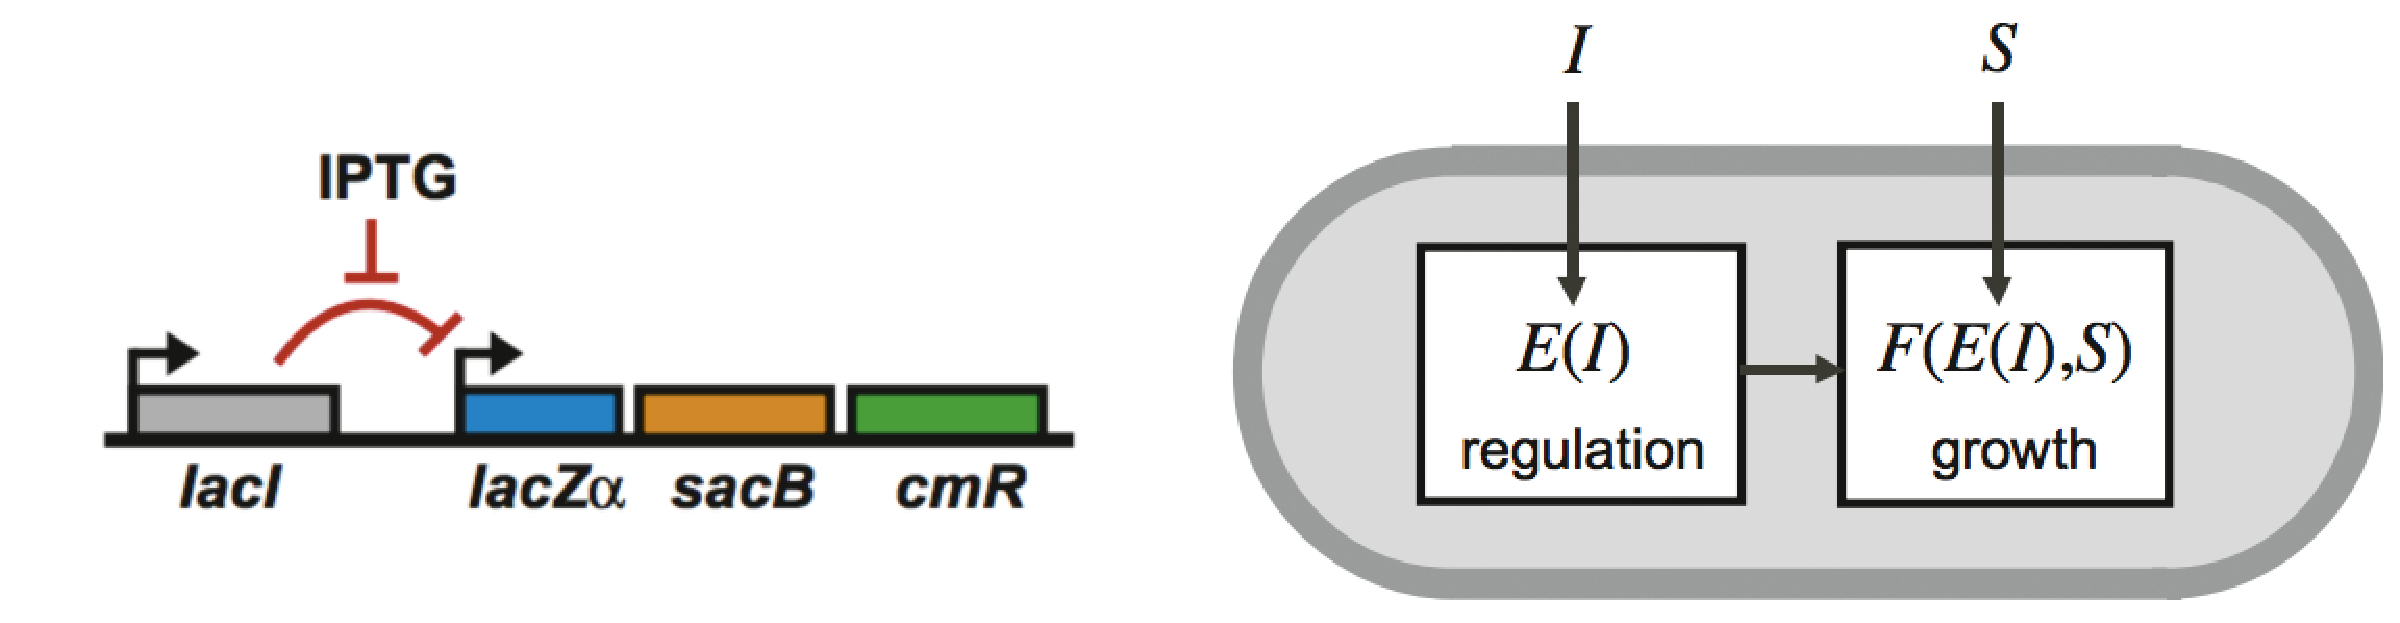
\includegraphics[width=0.7\textwidth]{poelwijk_design.pdf}
\end{center}

Poelwijk et al. (2011) created a synthetic construct in which an operon ``E" containing \textit{lacZ} (here, used as a marker), \textit{sacB}, and \textit{cmR} is regulated by the \textit{lac} repressor, LacI. By varying the concentration of IPTG (an analog of allolacose), the authors can experimentally control the expression level of this operon. In media containing chloramphenicol, expression is beneficial, and in media containing sucrose, it is deleterious, as expected.

\begin{center}
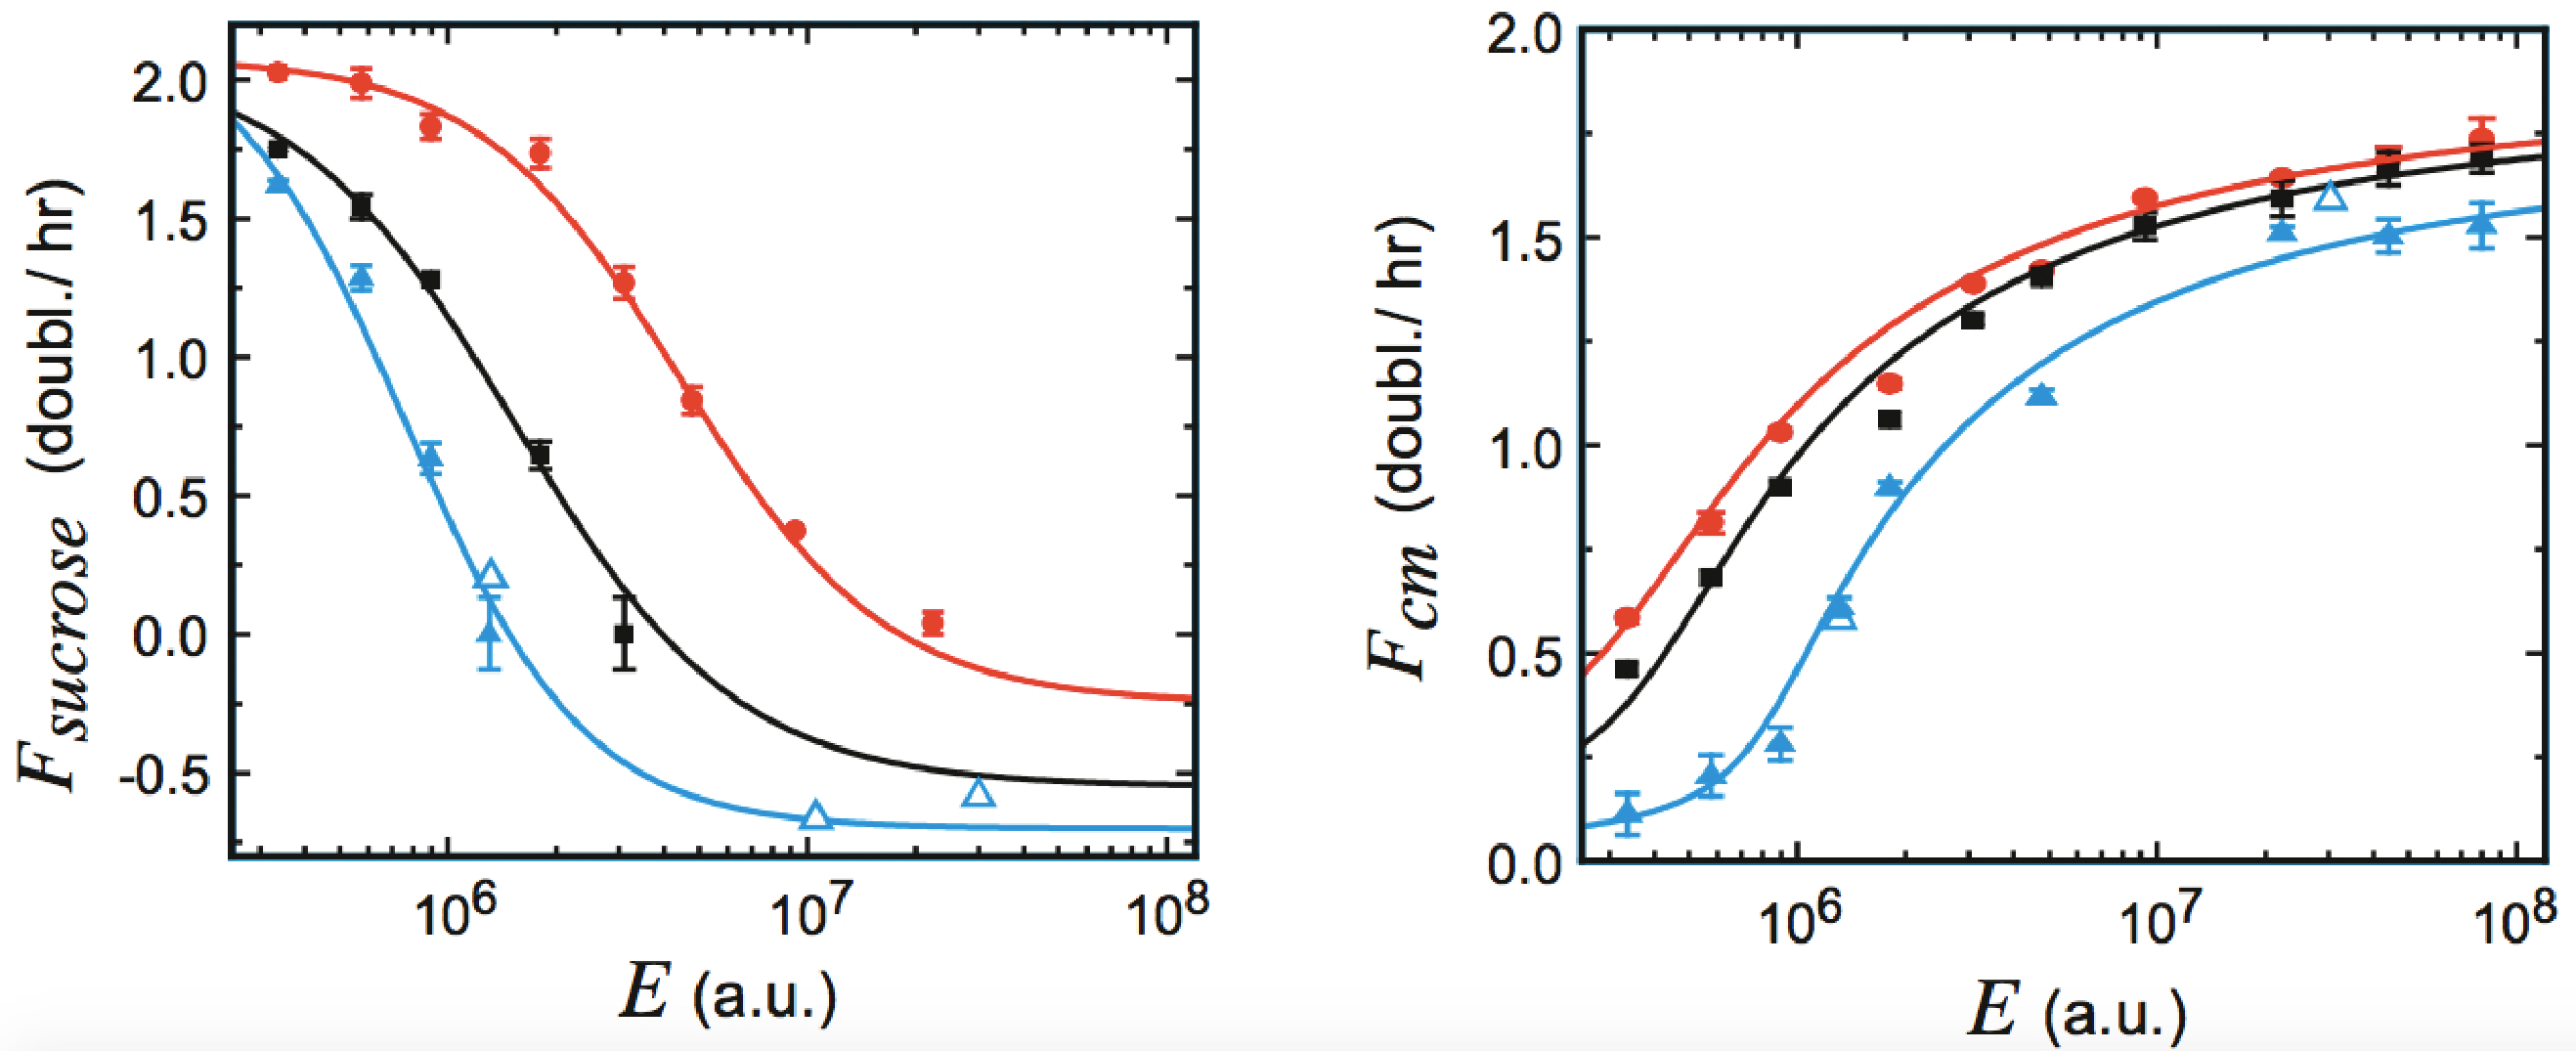
\includegraphics[width=0.7\textwidth]{fitness_vs_expression.pdf}
\end{center}

Suppose now that cells spend a fraction $p$ of their time in chloramphenicol and the rest in media containing sucrose. If a single expression level of E must be chosen (i.e. if the operon's expression is not regulated), then there are trade-offs between growth in the two environments. By plotting the strain's fitness in each type of media for different E expression levels (IPTG concentrations), the authors can examine the type of trade-off curve. If the curve is concave down, then the optimal solution is an intermediate level of expression so that growth will be mediocre in both environments. If the curve is concave up, however, the optimal strategy is to either to express E very highly or not at all -- essentially, to accept virtually nil growth under one condition and maximize growth under the other (Levins, 1968). Poelwijk et al. are able to find both types of trade-off curve in their system: the trade-off is concave down when both sucrose and chloramphenicol concentrations are low, and concave up when both concentrations are high.

\begin{center}
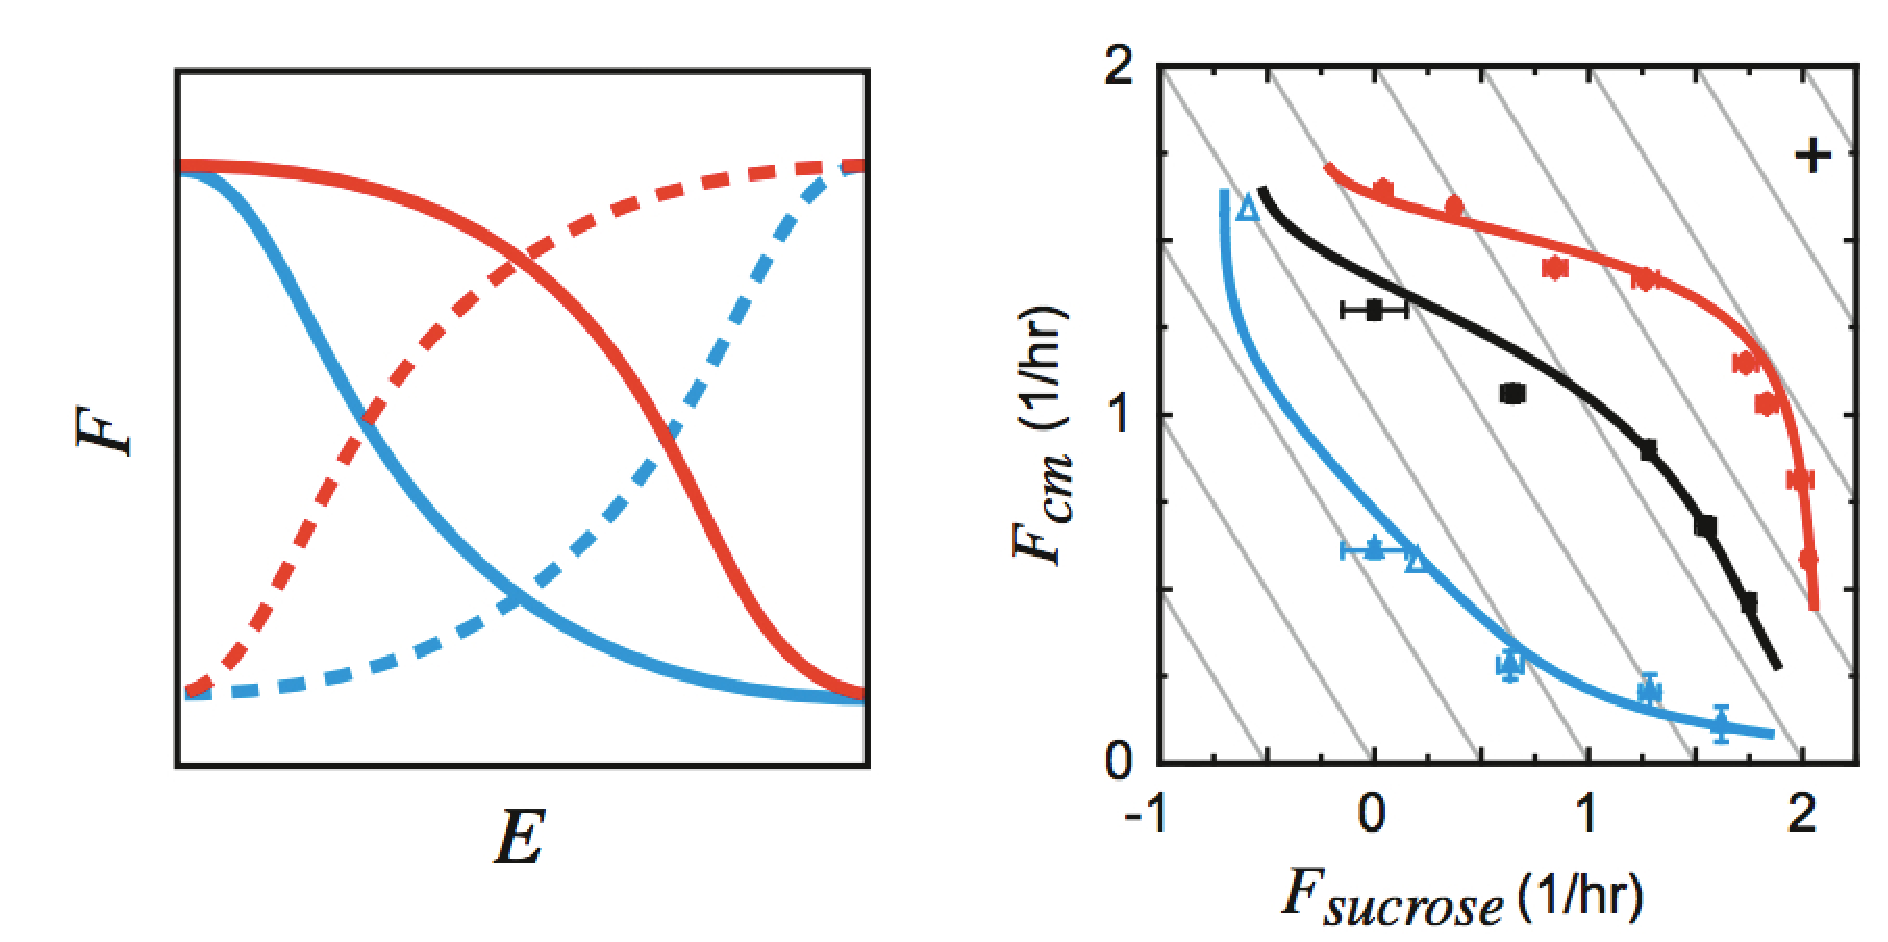
\includegraphics[width=0.7\textwidth]{tradeoff_curves.pdf}
\end{center}

Any steady-state regulatory pattern can be mimicked in this system simply by adjusting the concentration of IPTG in chloramphenicol vs. sucrose media accordingly. By comparing the fitness of the ``regulated" vs. ``unregulated" system, we can determine how much benefit would be derived from regulation of that type. This is the cost that the cell should be ``willing to pay" (e.g.in expenditure of energy) to maintain a regulatory system with that functionality\footnote{This statement should be interpreted as a prediction that regulation will not exist when the costs are greater than the potential benefits. There is of course no guarantee that a regulation system will evolve when it would be beneficial, though we will see that this is no great challenge on evolutionary or even experimental timescales to acquiring a new or altered regulatory system. This calculation also does not take into account the fitness effects due to transitions between environments.}.

\begin{center}
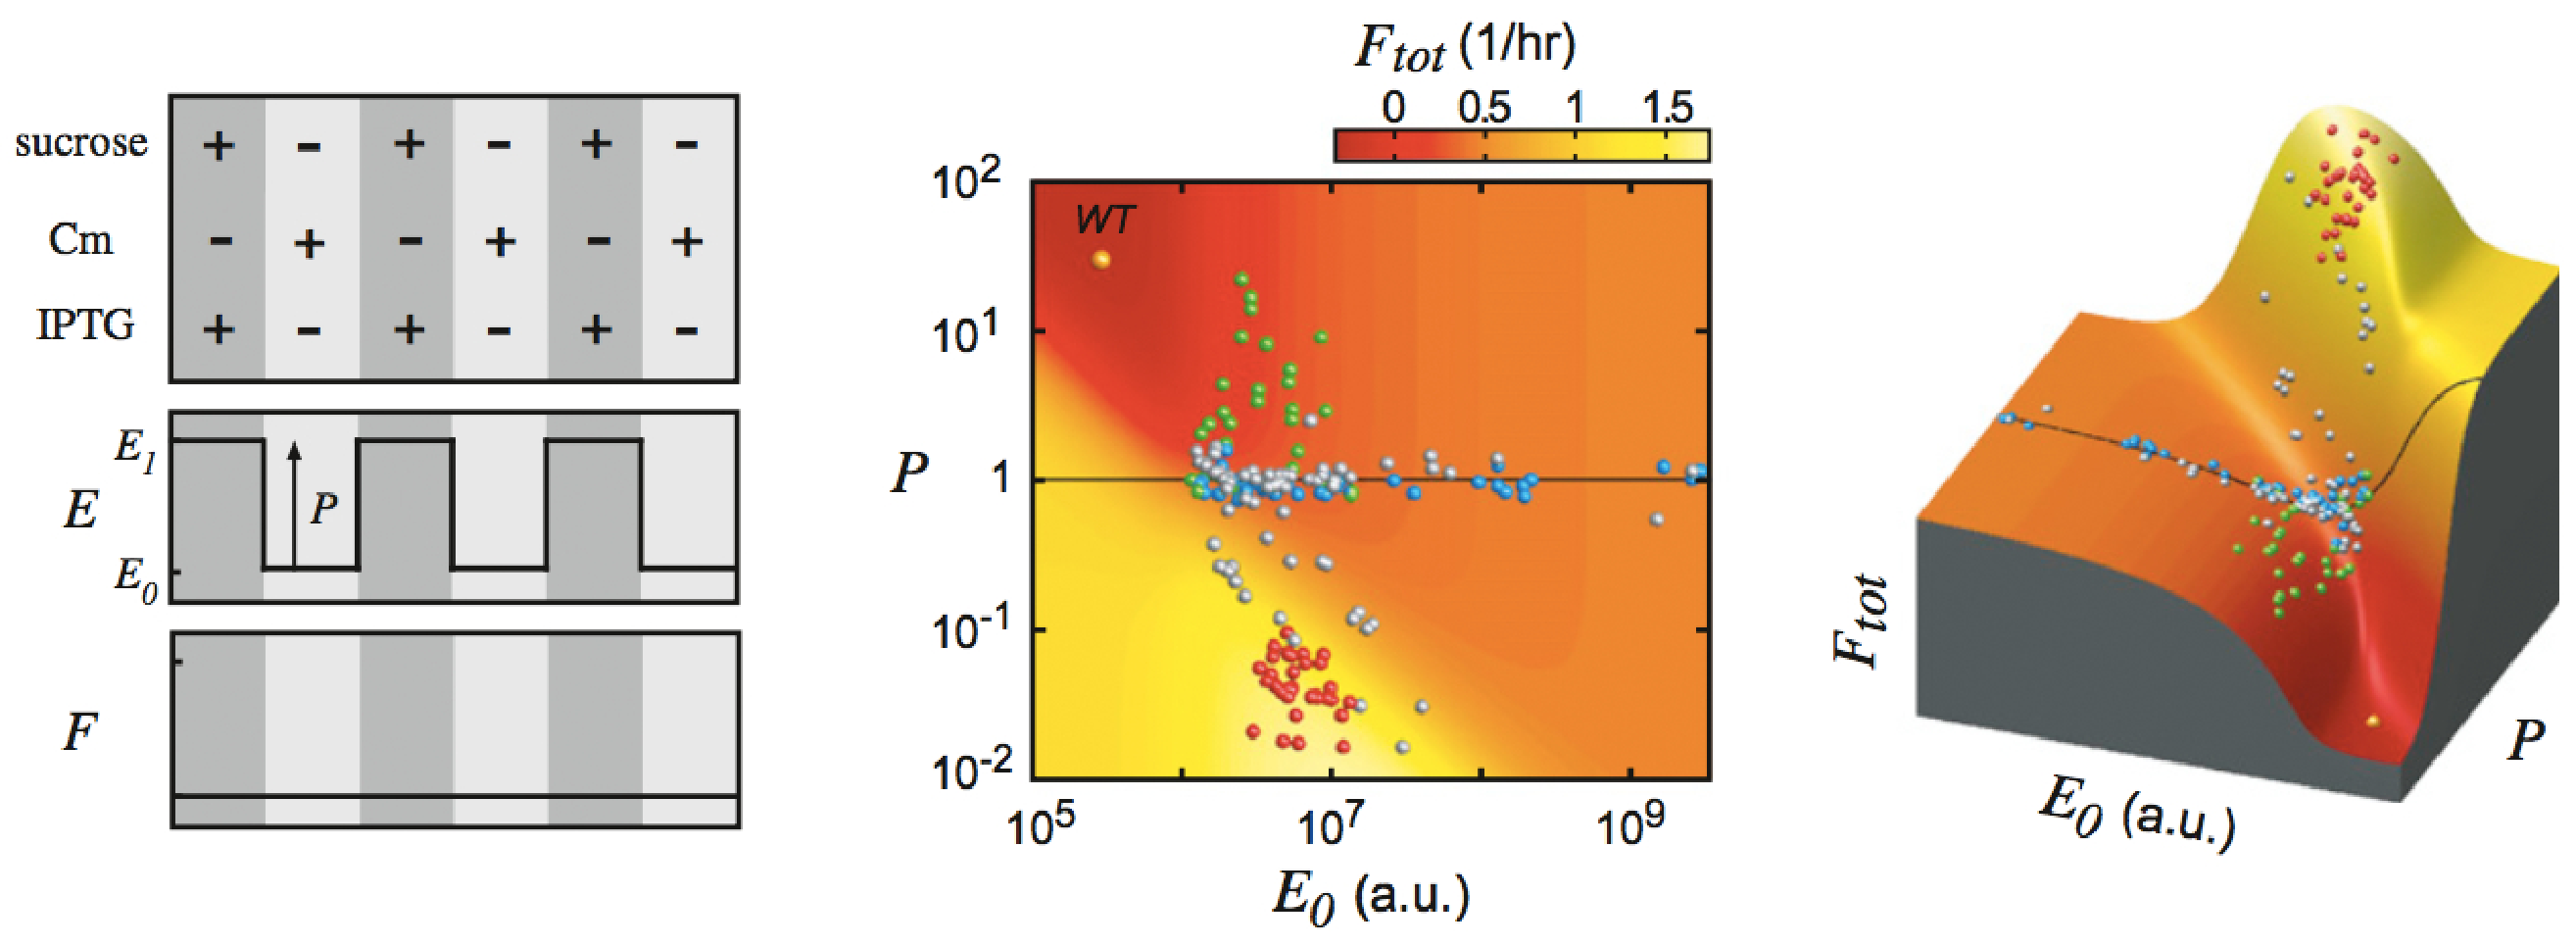
\includegraphics[width=\textwidth]{exp_evol_tans.pdf}
\end{center}

One way to assess whether it is ``difficult" for the optimal regulatory strategy to evolve is through artificial selection. The authors passaged the strain described above through alternating environments of chloramphenicol alone and IPTG + sucrose together -- conditions under which the starting construct was not ideal. They found that LacI could indeed be evolved to respond to IPTG by binding the operon more tightly, providing a case study where regulation is evolutionarily labile.

\section*{Thresholding vs. graded responses}

As an example of a cost-benefit analysis, consider an enzyme $E$ which converts a useless substrate $S$ (held at fixed concentration) into a useful product $P$ (Sivak and Thomson, 2014). If the enzyme obeys Michaelis-Menten kinetics, then the benefit is proportional to the rate of product formation:
\[ \textrm{ Benefit: } \frac{k_{cat} \left[ E \right] \left[ S \right] }{K_m + \left[ S \right] } \]
One potential cost is the enzyme's production: if the enzyme is simply regulated, then this cost simply scales with the steady-state concentration of the enzyme. Other costs might scale differently with the steady-state concentration of enzyme, so we will assume that the cost function is $\propto [E]^n$, where $n>1$ gives a concave up cost function, etc.

\begin{center}
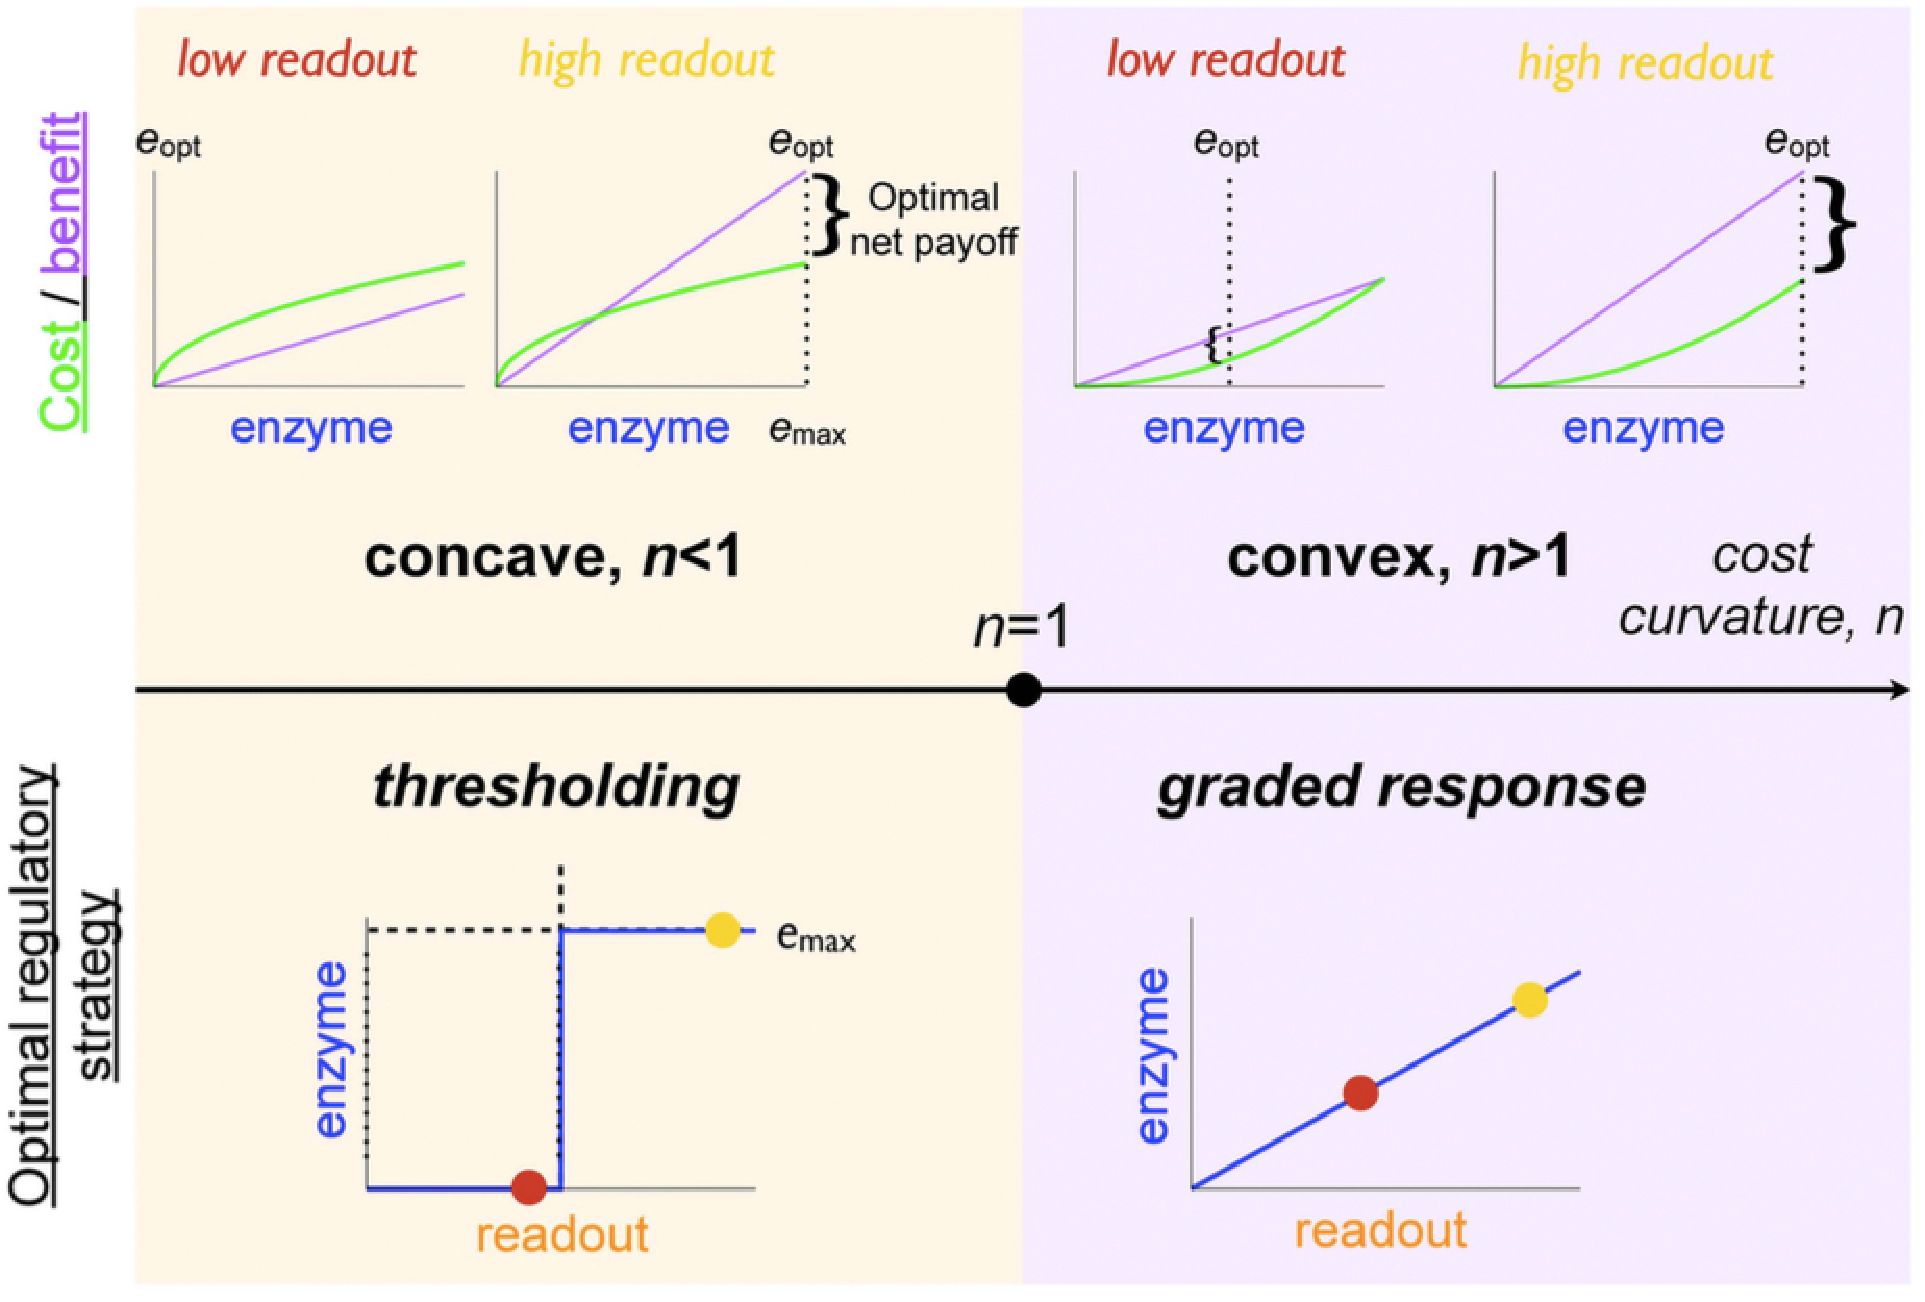
\includegraphics[width=0.8 \textwidth]{sivak1.pdf}
\end{center}


If $n<1$, it is possible that the cost function will lie completely above the benefit function, i.e., the ideal enzyme concentration will be zero. Raising the substrate concentration could change this, however, at which point the ideal enzyme concentration would become infinite: speaking more practically, the cell should make as much enzyme as it is able. If, however, $n>1$, then the ideal enzyme concentration will be intermediate and increasing with $S$. (If the enzyme stays in its first-order regime, then the optimal enzyme concentration will scale linearly with $S$.)  A straightforward interpretation is that when the cost function is concave down, the enzyme's production should be regulated in an all-or-none manner; otherwise, its production should scale with $S$:
\begin{eqnarray*}
0 = \frac{d \, \textrm{Profit}}{d\left[ E \right]} & = & \frac{d}{d\left[ E \right]} \left[  \frac{k_{cat} \left[ E \right] \left[ S \right] }{K_m + \left[ S \right] } -  c \left[ E \right]^n \right]\\
& \approx & \frac{d}{d \left[ E \right]} \left[ \frac{k_{cat} \left[ E \right] \left[ S \right] }{K_m} -  c \left[ E \right]^n  \right]\\
& = & \frac{k_{cat} \left[ S \right] }{K_m} -  c n \left[ E \right]^{n-1}\\
 \left[ E \right]_{\textrm{opt}} & = & \left( \frac{k_{cat} \left[ S \right]}{c n K_m} \right)^{\frac{1}{n-1}} \\
\end{eqnarray*}
This response assumes that the cell is able to measure [S] with infinite accuracy in order to select an enzyme expression level. If the mode of measurement is imperfect, a better guess for the true value of [S] might take into consideration not just the measured value, [S]$^*$, but also the prior probability of encountering a certain [S]:
\[ \textrm{E} \left( s \, | \,s^* \right) = \int s  P\left( s \, | \, s^* \right) \, ds =  \int \frac{ s P\left( s^* \, | \, s \right)P\left( s \right)}{P \left( s^* \right)} \, ds\]
where we have applied Bayes rule to the probability within the integrand. For example, if the true distribution of [S] is a Gaussian with mean $\mu$ and variance $\sigma_s^2$, and the measurement $s^*$ is a normally-distributed around $s$ with variance $\sigma_m^2$, then:
\begin{eqnarray*}
P\left( s^* \, | \, s \right) & \propto & \exp \left( -\frac{\left(s - s^*\right)^2}{2\sigma_m^2} \right)\\
P\left( s \right) & \propto & \exp \left( -\frac{\left(s - \mu\right)^2}{2\sigma_s^2} \right)\\
 \textrm{E} \left( s \, | \,s^* \right)  & = & \frac{s^*}{1+r} + \frac{r \mu}{1 + r}, \hspace{2 cm} r \triangleq \frac{\sigma_m^2}{\sigma_s^2}
\end{eqnarray*}
This result fits our intuition that the worse the measurement becomes, the less weight it should carry in an estimate of the true value of [S]. However, the expectation above can only be calculated if the cell ``knows" something about the relative variabilities of the measurement and [S], as well as the mean of the prior probability distribution of [S]. Most college graduates would have difficulty reckoning these quantities with a graphing calculator: how can an organism acquire and properly use this information? One possibility is that the mean value of [S] and the relative weighting of measured and prior values are hard-coded genetically into the regulatory system: the second term in the expression above could represent the ``basal" activity of the promoter, and the first term the sensitivity to the measured value [S]$^*$. ``Memory" of the prior probability distribtuon and relative variances would be encoded in $\mu$ and $r$ by mutation and selection for appropriate values of these parameters over long times.

\section*{Optimality in the presence of alternative strategies}

It is often the case that a regulatory strategy which would be ideal in isolation becomes untenable when organisms with alternative strategies are also present. This principle is well-captured by the famous Prisoner's Dilemma, and also experienced by the mice in J. Maynard Smith's haystacks (though in their case a cooperative strategy is maintained via population structure). A strategy is called evolutionarily stable if a population exhibiting it would be able to fend off any alternative strategy that might appear within it. In other words, an evolutionarily stable strategy (ESS) will be maintained in the face of mutation and selection.\\

The concept of the ESS was first described by J. Maynard Smith and George Price in a \textit{Nature} paper called ``The logic of animal conflict," which they modeled using a multi-round variation on the Prisoner's Dilemma, allowing strategies that exacted vengeance for failure to cooperate or ended interactions early. They proposed a few strategies with varying levels of aggression and vindictive tendencies and simulated how these strategies would fare against one another. In 1980, Robert Axelrod expanded on this work by hosting a round-robin tournament in which game theorists were invited to submit programs that enacted any strategy they desired, and these programs were pitted against one another. The winner was Anatol Rapoport's TIT FOR TAT which cooperated with its opponent only when the opponent cooperated as well, effectively implementing ``justice."\\

Unfortunately it is not always possible to penalize unfair players or retreat from them. Moreover, ``cheaters" that fail to exhibit a cooperative strategy appear often in nature, even in communities that have very low genetic diversity. A classic example is cancer, where the failure of a cell to limit its own growth can result in the death of the organism. As in the haystack model, population structure prevents cancerous cells from rising in frequency above a certain fraction: these cells (typically) cannot be transferred between individuals or form new individuals.\\

The importance of this structure is evident in light of the decimation of the Tasmanian devil population by a transmissible oral cancer. First identified in 1996 by a photographer, the cancer has now rapidly spread across most of the island: more than 80\% of wild devils are infected. Tasmanian devils bite one another while engaging in mating battles and roughhousing. The low genetic diversity of Tasmanian devils, particularly at Major Histocompatibility Complex (MHC) loci -- the same that are genotyped when identifying potential organ donors -- prevents the host's immune system from recognizing the cancer cells as foreign.\\

A strategy that is optimal in isolation but not evolutionarily stable is expected to be lost on long timescales unless some mitigating factor ensures that organisms with the same strategy are more likely to interact with one another than is expected by chance. Most forms of population structure -- growth of colonies or multicellular organisms from a single cell, even random assortment into small groups as seen with J. Maynard Smith's haystack model -- have the potential to stabilize such strategies. When spatial segregation cannot be reliably arranged, ``reputation" systems can be used to help organisms identify and interact with those who share similar strategies.\\

``Green beard" genes, so named by Richard Dawkins (1976) but originally proposed by Hamilton (1964), represent an especially simple form of reputation system. These genes produce an obvious phenotype that is closely associated with a certain behavioral pattern, namely, cooperation with others who possess the same gene. The green beard gene only works as long as the behavior is well-correlated with the phenotype. For example, MIT graduates frequently wear enormous brass rats by which they easily recognize one another in their business dealings and hiring interviews, and on the whole they are less likely to treat each other unfairly out of a sense of kinship. However it is for anyone with larcenous inclinations to obtain such a ring and thus benefit from these insider deals without necessarily paying it forward. One therefore should be concerned with how frequently behavioral mutants might arise and how closely these two traits are associated.\\

In some very particular cases, it is possible to functionally link the green beard phenotype to its cooperative function. The \textit{FLO1} gene in \textit{S. cerevisiae} provides an excellent example (Smukalla et al., 2008). In response to high ethanol concentrations, yeast begin to express cell surface flocculation proteins that help them to stick to any other cells expressing the same proteins. The result is that a portion of cells become encased in the remainder and thus protected from exposure to the high ethanol concentrations. Cells that ``cheat" by expressing less \textit{FLO1} tend to wind up at the periphery (or not in the floc at all) because they do not interact as strongly with other cells.


\section*{Genetically-encoded ``prediction"}

You have seen that circadian rhythms have evolved multiple times independently. We have argued that these clocks allow organisms to begin prepare for anticipated conditions without the delay required by a ``reactionary" regulatory system. Regulatory systems that predict upcoming events do not need to be as intricate as circadian clocks. For example, \textit{E. coli} thrives in the mammalian gut: its life cycle includes phases in which the bacterium lives outside of its host, at colder temperatures but with greater exposure to oxygen. An increase in temperature may signal re-ingestion and resulting decrease in oxygen availability: it has been found that transcriptional responses to increase in temperature mimic those due to decrease in oxygen availability (Tagkopoulos et al., 2008), so that the cell may be envisioned to anticipate the oncoming change in oxygen levels as soon as it senses rising temperature.\\

Similarly, \textit{E. coli}'s path through the intestine takes it through regions in which the availability of sugars is quite different: lactose is available primarily in the early small intestine, while maltose remains available untill much later.  Lactose exposure in \textit{E. coli} is capable of inducing both the \textit{lac} operon and (to a lesser extent) maltose metabolism operons, which in a sense prepares the cell to transition to the latter sugar. Maltose, however, induces only maltose operons. When \textit{E. coli} are evolved in the lab where this sequence of environments is not experienced, the ability of lactose to induce maltose operons is rapidly lost (Mitchell et al., 2009).\\

A related effect is also observed in yeast. Grape must undergoing fermentation produces caricatured changes in extracellular environment beginning with exposure to a high osmolarity and a (partially yeast-induced) low pH, followed by increase in temperature and ethanol concentration due to the yeast's metabolic activity, and finally oxidative stress caused by the transition from fermentation to respiration as simple sugars are depleted. Heat and ethanol stresses induce responses that protect cells from oxidative stress (Mitchell et al., 2009).

\end{document}